%
% main.tex
%
% Copyright (C) 2022 by Universidade Federal de Santa Catarina.
%
% GNSS Networks Based on Small Satellites
%
% This work is licensed under the Creative Commons Attribution-ShareAlike 4.0
% International License. To view a copy of this license,
% visit http://creativecommons.org/licenses/by-sa/4.0/.
%

%
% \brief Main file.
%
% \author Gabriel Mariano Marcelino <gabriel.mm8@gmail.com>
%
% \version 0.1.0
%
% \date 2019/11/30
%

\documentclass[journal]{IEEEtran}

\usepackage{article}

\title{GNSS Networks Based on Small Satellites}
\author{Gabriel M. Marcelino, Eduardo A. Bezerra
	\thanks{
	Gabriel Mariano Marcelino, UFSC, Brazil, (email: \href{mailto:gabriel.marcelino@spacelab.ufsc.br}{gabriel.marcelino@spacelab.ufsc.br})

	Eduardo A. Bezerra, UFSC, Brazil, (email: \href{mailto:eduardo.bezerra@ufsc.br}{eduardo.bezerra@ufsc.br})
	}}
\date{}

\hypersetup
{
    pdfauthor   = {Gabriel Mariano Marcelino},
    pdfsubject  = {PhD Thesis Qualification},
    pdftitle    = {GNSS Networks Based on Small Satellites},
    pdfkeywords = {Embedded Systems,GNSS,Satellites}
}

\begin{document}

    \maketitle

    \begin{abstract}
        Abstract...
    \end{abstract}

    \begin{IEEEkeywords}
        Embedded Systems, GNSS, Satellites.
    \end{IEEEkeywords}

    %
% introduction.tex
%
% Copyright (C) 2021 by Universidade Federal de Santa Catarina.
%
% On-Board Data Processing Techniques to Improve the Performance of Small Satellites
%
% This work is licensed under the Creative Commons Attribution-ShareAlike 4.0
% International License. To view a copy of this license,
% visit http://creativecommons.org/licenses/by-sa/4.0/.
%

%
% \brief Introduction section.
%
% \author Gabriel Mariano Marcelino <gabriel.mm8@gmail.com>
%
% \version 0.0.0
%
% \date 2019/11/30
%

\section{Introduction} \label{sec:introduction}


Possíveis aplicações:

\begin{itemize}
    \item Detecção de eventos
    \item Detecção e alerta de desastres naturais: alertas vindo diretamente do satélite podem ser maís rápidos que enviar dados coletados e processar em terra.
    \item Vigilância: eventos podem ser detectados em tempo real e alertas enviados para lugares específicos (drones, estações, etc.)
    \item Aplicações militares
\end{itemize}

    %
% related-work.tex
%
% Copyright (C) 2022 by Universidade Federal de Santa Catarina.
%
% GNSS Networks Based on Small Satellites
%
% This work is licensed under the Creative Commons Attribution-ShareAlike 4.0
% International License. To view a copy of this license,
% visit http://creativecommons.org/licenses/by-sa/4.0/.
%

%
% \brief Related works section.
%
% \author Gabriel Mariano Marcelino <gabriel.mm8@gmail.com>
%
% \version 0.0.0
%
% \date 2021/06/14
%

\section{Related Work} \label{sec:related-work}

\subsection{Current GNSS networks}

Atualmente existem N redes de GNSS em operação, X em fase de implantação e testes e Y redes em planejamento.

Abaixo, encontra-se uma descrição de cada uma dessas redes.

\subsubsection{GPS}

\subsubsection{GLONASS}

O GLONASS, sigla de \textit{Globalnaya navigatsionnaya sputnikovaya sistema} (ou Sistema de Navegação Global por Satélite), é o sistema de GNSS criado e mantido pela Rússia.

\subsubsection{Galileo}

O Galileo é o sistema de GNSS criado pela união europeia.

\subsubsection{BeiDou}

BeiDou, ou \textit{BeiDou Navigation Satellite System} (BDS) é o sistema de GNSS chinês.






A \autoref{tab:gnss-networks} compara as principais características dos sistemas de GNSS apresentados acima.


\cite{aarestad2020}

\begin{figure}[!ht]
    \begin{center}
        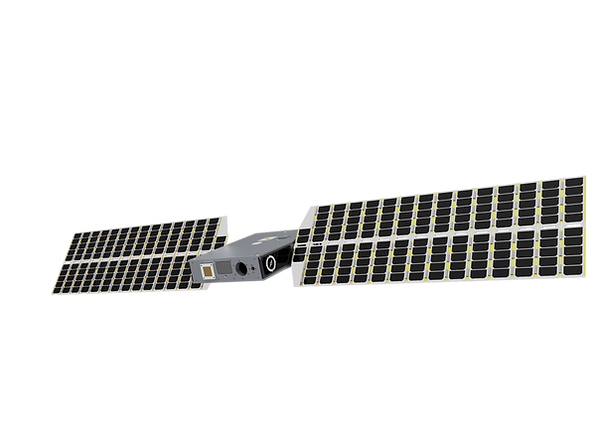
\includegraphics[width=\columnwidth]{figures/xona-satellite}
        \caption{Xona Space Systems conceptual satellite.}
        \label{fig:xona-satellite}
    \end{center}
\end{figure}

\subsection{Experimental GNSS networks}

    %
% problem-discussion.tex
%
% Copyright (C) 2021 by Universidade Federal de Santa Catarina.
%
% On-Board Data Processing Techniques to Improve the Performance of Small Satellites
%
% This work is licensed under the Creative Commons Attribution-ShareAlike 4.0
% International License. To view a copy of this license,
% visit http://creativecommons.org/licenses/by-sa/4.0/.
%

%
% \brief Problem discussion section.
%
% \author Gabriel Mariano Marcelino <gabriel.mm8@gmail.com>
%
% \version 0.1.0
%
% \date 2021/06/14
%

\section{Problem Discussion} \label{sec:problem-discussion}

\cite{marcelino2018}

\cite{marcelino2016}

\begin{itemize}
    \item IA embarcada
    \item Voo em formação
    \item Constelação de nanossatélites
    \item Processamento distribuído (constelação)
\end{itemize}

\subsection{Processing Hardware}

\begin{itemize}
    \item Nvidia Jetson
    \item Intel Movidius
    \item FPGA
\end{itemize}

\subsection{Descrição de hardware}

Guppy GPU \cite{al-dujaili2012}

NOEL-V \cite{andersson2020}

RISC-V \cite{waterman2016}

    %
% proposed-work.tex
%
% Copyright (C) 2021 by Universidade Federal de Santa Catarina.
%
% On-Board Data Processing Techniques to Improve the Performance of Small Satellites
%
% This work is licensed under the Creative Commons Attribution-ShareAlike 4.0
% International License. To view a copy of this license,
% visit http://creativecommons.org/licenses/by-sa/4.0/.
%

%
% \brief Proposed work section.
%
% \author Gabriel Mariano Marcelino <gabriel.mm8@gmail.com>
%
% \version 0.1.0
%
% \date 2021/06/14
%

\section{Proposed Work} \label{sec:proposed-work}

\begin{itemize}
    \item Explorar técnicas e métodos para aumentar a capacidade de proessamento embarcado em pequenos satélites
    \item Explorar técnicas de redução do consumo de energia durante o processamento, e consequentemente a eficiência energética do computador de bordo
    \item Para isso, levar em consideração as questões ambientais da operação de um satélite, como a incidência de radiação, que degrada o funcionamento de toda a eletrônica embarcada
    \item \textcolor{blue}{Previsão do tempo e desastres direto no satélite, transmitindo alertas direto para dispositivos em Terra (smartphones?)}
\end{itemize}

\subsection{FloripaSat-2 Experiment}

Como um primeiro experimento para aplicar os conceitos aqui apresentados, pretende-se executar um experimento a ser embarcado no nanossatélite FloripaSat-2 \cite{floripasat2}.

The Radiation Monitor (or Harsh Payload) is a payload capable of evaluate the radiation effects on three SDRAM memories with different manufacturing nodes. This payload will test this chips in the real harsh space environment by flying aboard of FloripaSat-2 CubeSat mission. These particular SDRAM memories were previous characterized on laboratory experiments, then by exposing them to the real environments and executing the same tests routines will not only generate more results for analysis, but also provide an opportunity to assess the test methodologies themselves. Also, after collecting sufficient data to be analysed, this payload could be used to provide a meaningful health status, concerning the radiation doses which the satellite were exposed, to the entire satellite subsystems and further missions. A picture of the harsh payload board is available in \autoref{fig:harsh-payload-pcb}.

\begin{figure}[!ht]
    \begin{center}
        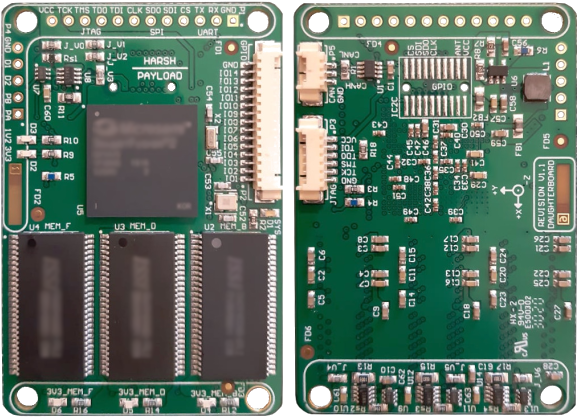
\includegraphics[width=0.8\columnwidth]{figures/harsh-payload}
        \caption{Harsh payload PCB.}
        \label{fig:harsh-payload-pcb}
    \end{center}
\end{figure}

\begin{figure}[!ht]
    \begin{center}
        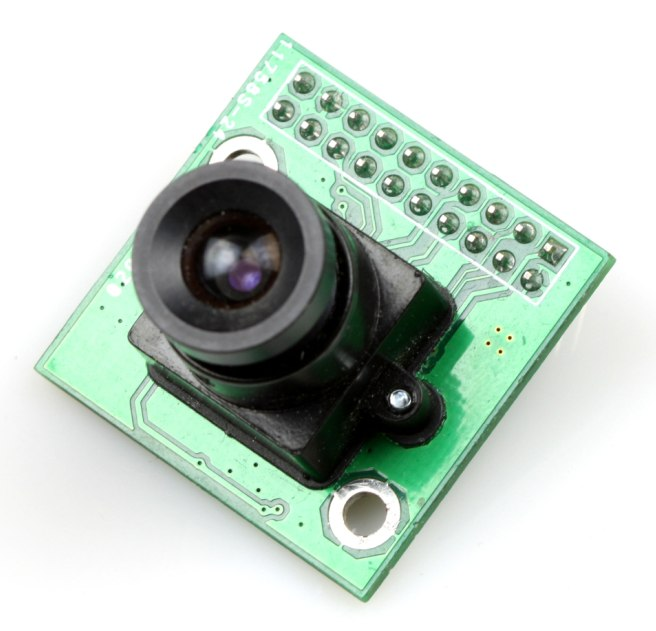
\includegraphics[width=0.5\columnwidth]{figures/mt9d111-m12}
        \caption{Arducam camera module (MT9D111 sensor).}
        \label{fig:mt9d111-module}
    \end{center}
\end{figure}

\begin{figure}[!ht]
    \begin{center}
        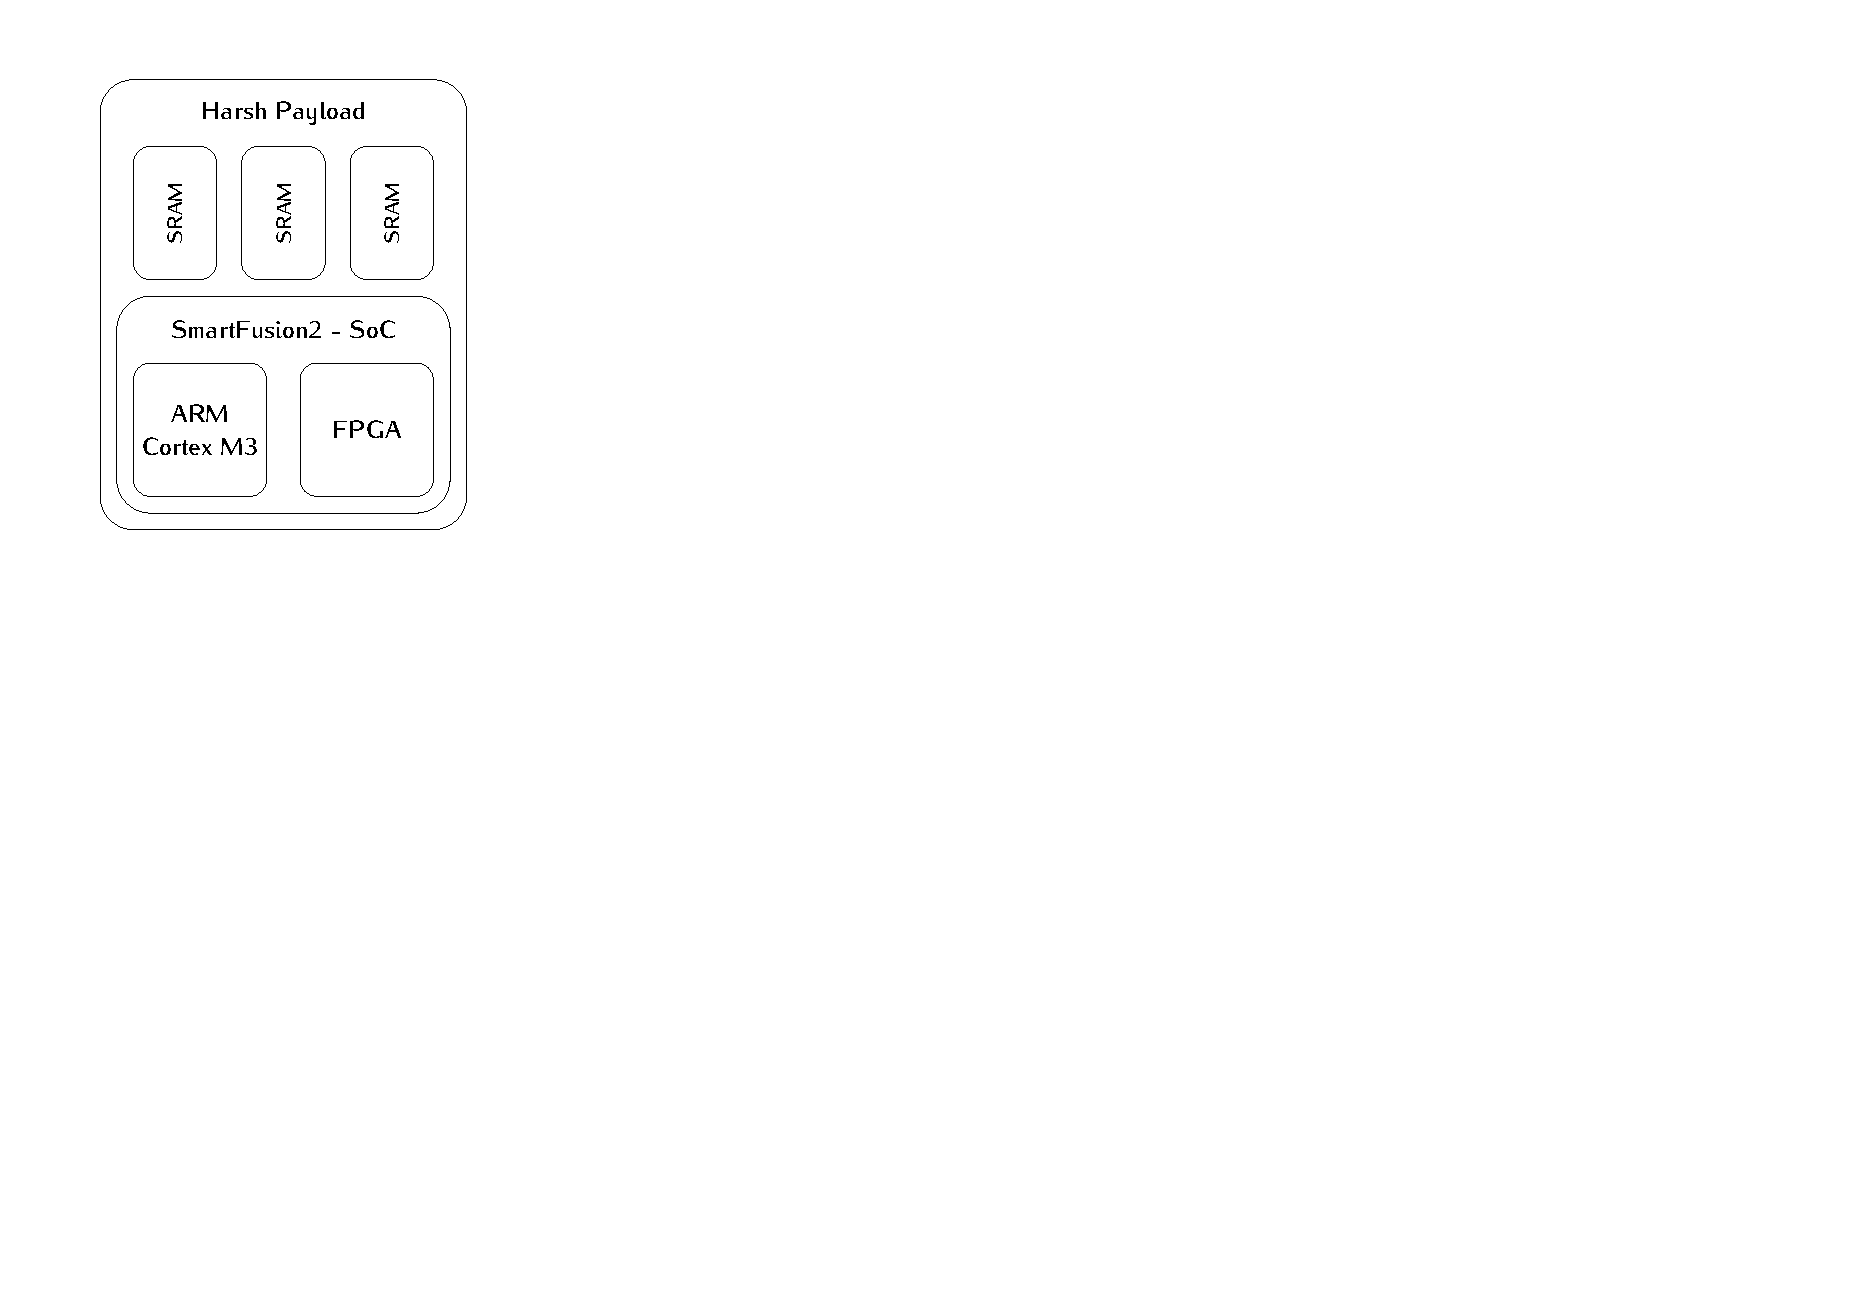
\includegraphics[width=0.5\columnwidth]{figures/harsh-block-diagram}
        \caption{Block diagram of the platform to be used in the proposed experiment.}
        \label{fig:experiment-platform-block-diagram}
    \end{center}
\end{figure}

%In order to accomplish this objectives, the payload is designed to follow the OBDH DaughterBoard standard of SpaceLab, which defines the connectors, shape and size of the board. This standard allows the utilization of the module throughout future SpaceLab core missions in reason of its low space occupation inside the CubeSat, being considered further as an expansion module instead of a payload experiment. A picture of the exploded view of the harsh payload and the OBDH can be seen in \autoref{fig:harsh-payload-integration}.

Also, due to the mission limited power budget, the developed board should consider reduce power consumption and define clever power management strategies. In addition, methods for anti latch-up, a type of short circuit which can occur inside an IC, are considered in the design. Therefore, combining all these requirements, the payload architecture consists of the following modules: a control and management subsystem, operated by a System-On-a-Chip (SoC) solution with an integrated FPGA, power converters for properly voltage level supply, anti latch-up circuitry, communication and interface buses, debug module and the SDRAM memory chips.

\begin{figure}[!htb]
    \begin{center}
        \subfigure[Image example.\label{fig:var-filter-img}]{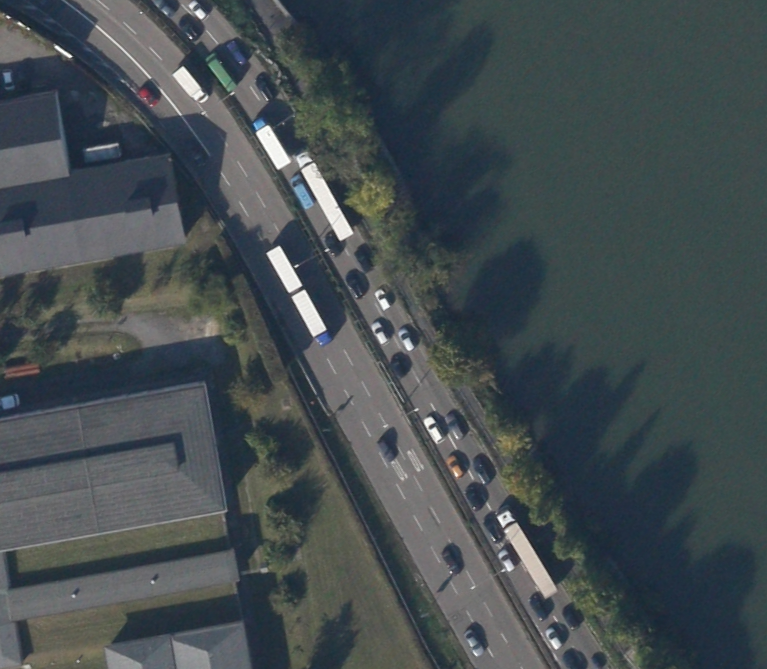
\includegraphics[width=\columnwidth]{figures/MOS15}}

        \subfigure[Variance filter result.\label{fig:var-filter-res}]{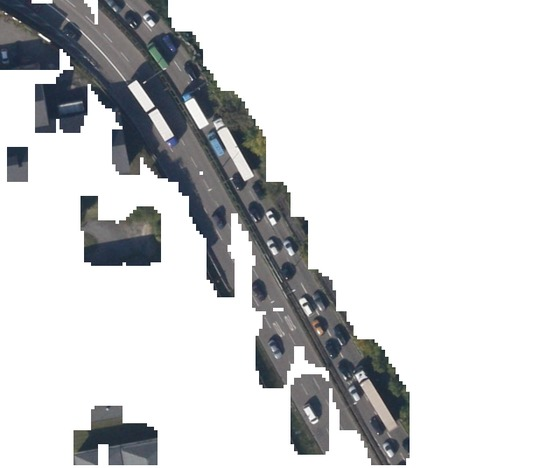
\includegraphics[width=\columnwidth]{figures/var-filter-output}}
        \caption{Variance filter example.}
        \label{fig:variance-filter-example}
    \end{center}
\end{figure}

\begin{figure*}[!ht]
    \begin{center}
        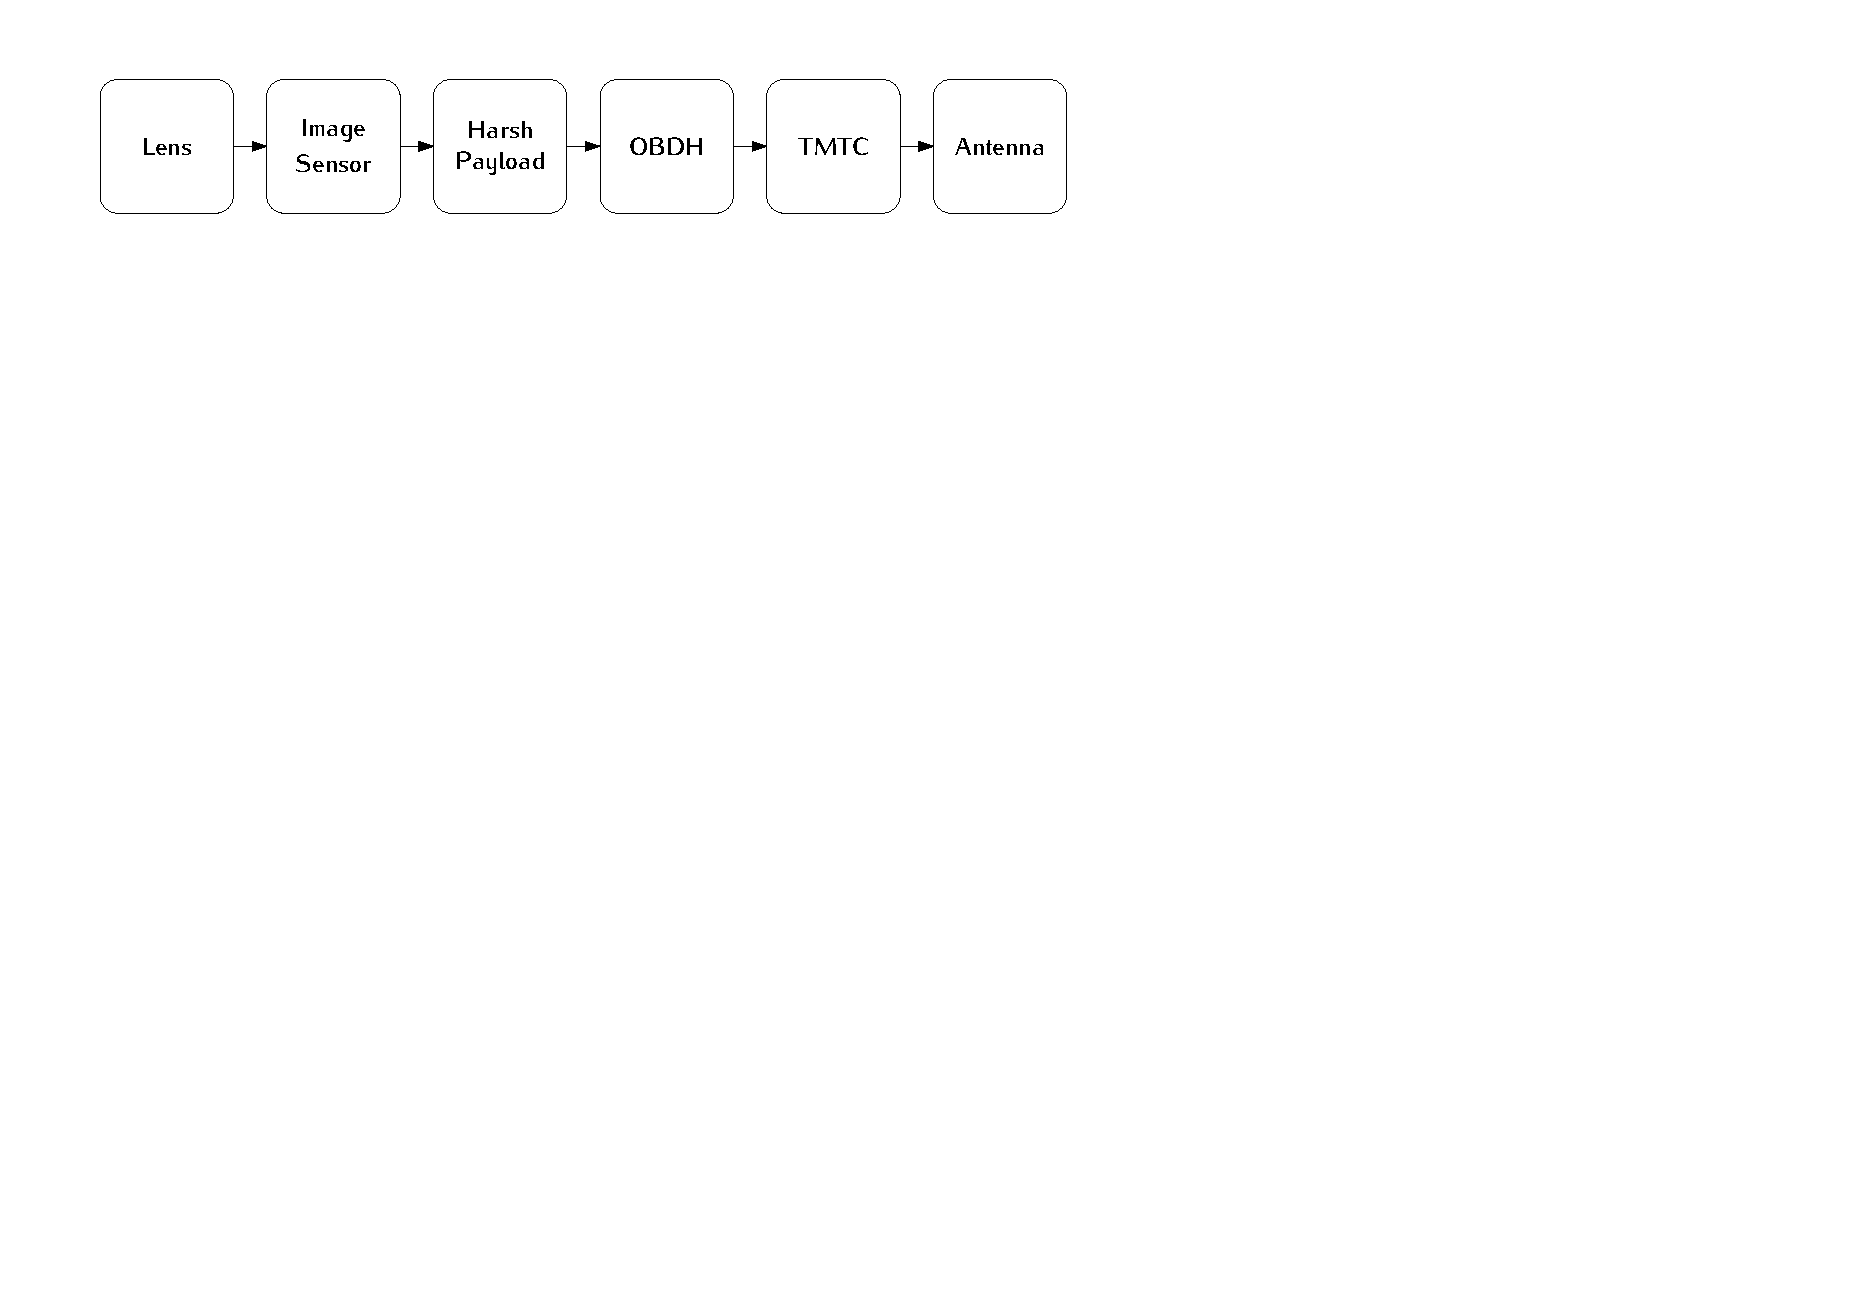
\includegraphics[width=0.8\textwidth]{figures/experiment-block-diagram}
        \caption{Block diagram of the experiment's hardware.}
        \label{fig:experiment-block-diagram}
    \end{center}
\end{figure*}


    %
% conclusion.tex
%
% Copyright (C) 2022 by Universidade Federal de Santa Catarina.
%
% GNSS Networks Based on Small Satellites
%
% This work is licensed under the Creative Commons Attribution-ShareAlike 4.0
% International License. To view a copy of this license,
% visit http://creativecommons.org/licenses/by-sa/4.0/.
%

%
% \brief Conclusion section.
%
% \author Gabriel Mariano Marcelino <gabriel.mm8@gmail.com>
%
% \version 0.0.0
%
% \date 2019/11/30
%

\section{Conclusion} \label{sec:conclusion}


    %
% acknowledgements.tex
%
% Copyright (C) 2022 by Universidade Federal de Santa Catarina.
%
% GNSS Networks Based on Small Satellites
%
% This work is licensed under the Creative Commons Attribution-ShareAlike 4.0
% International License. To view a copy of this license,
% visit http://creativecommons.org/licenses/by-sa/4.0/.
%

%
% \brief Acknowledgements section.
%
% \author Gabriel Mariano Marcelino <gabriel.mm8@gmail.com>
%
% \version 0.0.0
%
% \date 2019/11/30
%

\section*{Acknowledgements} \label{sec:acknowledgements}

    %
% references.tex
%
% Copyright (C) 2022 by Universidade Federal de Santa Catarina.
%
% GNSS Networks Based on Small Satellites
%
% This work is licensed under the Creative Commons Attribution-ShareAlike 4.0
% International License. To view a copy of this license,
% visit http://creativecommons.org/licenses/by-sa/4.0/.
%

%
% \brief References section.
%
% \author Gabriel Mariano Marcelino <gabriel.mm8@gmail.com>
%
% \version 0.1.0
%
% \date 2019/11/30
%

\bibliographystyle{unsrt}

\bibliography{references/floripasat2,%
              references/nanosatseu,%
              references/aarestad2020,%
              references/xona-space,%
              references/sa45s,%
              references/beidou,%
              references/glonass,%
              references/gps,%
              references/qzss,%
              references/irnss,%
              references/larson2005,%
              references/marino2016,%
              references/cds,%
              references/thombre2015,
              references/gps-standard}


\end{document}
